\documentclass[11pt]{article}

\usepackage[margin=1in]{geometry}
\usepackage{amsmath,amssymb,bm}
\usepackage{siunitx}
\usepackage{enumitem}
\usepackage{hyperref}
\usepackage{graphicx}
\usepackage{tikz}

\usetikzlibrary{arrows.meta,decorations.pathmorphing}

\hypersetup{
  colorlinks=true,
  linkcolor=blue,
  urlcolor=blue,
  citecolor=blue
}

\setlist[itemize]{leftmargin=*, itemsep=3pt}
\setlist[enumerate]{leftmargin=*, itemsep=6pt}

\newcommand{\dd}{\,\mathrm{d}}
\newcommand{\pd}[2]{\frac{\partial #1}{\partial #2}}

\begin{document}

\begin{center}
{\Large \textbf{MMAE 450 --- Homework \#3}}\\[4pt]
{\large \textbf{FTCS for Transient Heat Conduction: Verification and Sphere Cooling}}\\[6pt]
\textbf{Due: Tuesday, February 3, 2026 (11:59 pm)}\\
\end{center}

\vspace{0.5em}

\noindent\textbf{Learning goals.} By completing this assignment, you will:
\begin{itemize}
  \item implement the \textbf{Forward Time, Centered Space (FTCS)} method for diffusion,
  \item investigate the distinction between \emph{stability} and \emph{accuracy} for explicit time integration,
  \item enforce \textbf{Dirichlet}, \textbf{Neumann (zero flux)}, and \textbf{Robin (convection)} boundary conditions,
  \item apply FTCS to a physically meaningful cooling problem.
\end{itemize}

\hrule
\vspace{0.9em}

% =====================================================================
\section*{Problem 1: Code Verification on a 1D Rod (Dirichlet--Dirichlet)}

Before tackling the spherical cooling problem, you will verify your FTCS implementation on the
\emph{1D Cartesian heat equation}:
\begin{equation}
\pd{T}{t} = \alpha \pd{}{x}\!\left(\pd{T}{x}\right) = \alpha \frac{\partial^2 T}{\partial x^2},
\qquad 0<x<L,\ t>0.
\end{equation}

Use the following setup:
\[
L=\SI{0.10}{m},\qquad T_\mathrm{L}=\SI{100}{^\circ C},\qquad T_\mathrm{R}=\SI{20}{^\circ C}.
\]
Initial condition:
\[
T(x,0)=\SI{100}{^\circ C}.
\]
Boundary conditions (Dirichlet at both ends):
\[
T(0,t)=T_\mathrm{L},\qquad T(L,t)=T_\mathrm{R}.
\]

\subsection*{Material data}
Use copper properties throughout this assignment:
\[
k=\SI{401}{W/(m\cdot K)},\qquad
\rho=\SI{8960}{kg/m^3},\qquad
c_p=\SI{385}{J/(kg\cdot K)},\qquad
\alpha=\frac{k}{\rho c_p}.
\]

\subsection*{Tasks}
\begin{enumerate}
  \item Discretize the rod with $N+1$ nodes and $\Delta x=L/N$. Implement FTCS for the interior nodes:
  \[
  T_i^{n+1}
  =
  T_i^n + \lambda\left(T_{i+1}^n - 2T_i^n + T_{i-1}^n\right),
  \qquad
  \lambda=\frac{\alpha\,\Delta t}{\Delta x^2},
  \qquad i=1,\dots,N-1.
  \]
  Enforce the Dirichlet boundary values at \emph{every} time step.
  \item Choose at least three time steps $\Delta t$ (equivalently, three values of $\lambda$) including:
  \begin{itemize}
    \item one that is clearly stable,
    \item one that is close to the stability limit,
    \item one that is unstable.
  \end{itemize}
  \item For each run, plot:
  \begin{itemize}
    \item $T(x,t)$ profiles at several times,
    \item $T$ at the midpoint vs.\ time.
  \end{itemize}
  \item In 2--3 sentences, describe what you observe as $\Delta t$ increases (stability vs.\ accuracy).
\end{enumerate}

\hrule
\vspace{0.9em}

% =====================================================================
\section*{Problem 2: Cooling of a Copper Sphere (Neumann at Center, Convection at Surface)}

A solid copper sphere of radius $R=\SI{0.10}{m}$ is initially at a uniform temperature
$T_0=\SI{100}{^\circ C}$. At time $t=0$ the sphere is removed from an oven and exposed to still air at
$T_\infty=\SI{20}{^\circ C}$ with a constant convective heat transfer coefficient $h$.

\begin{center}
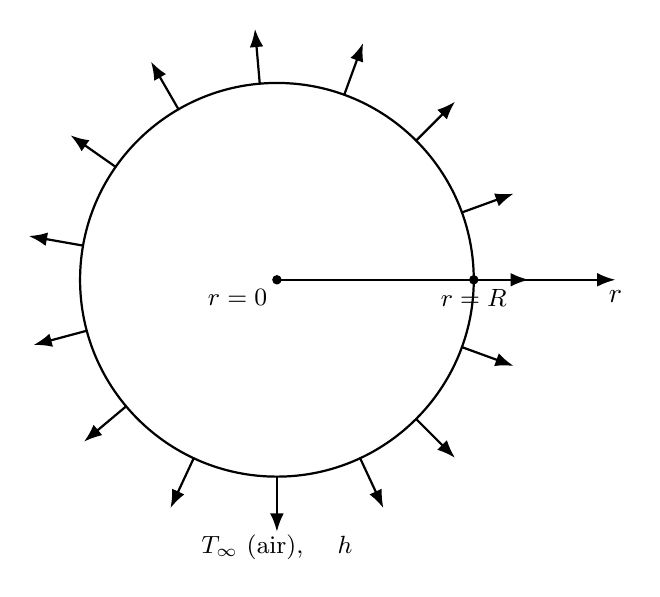
\begin{tikzpicture}[scale=2.0, line cap=round, line join=round]
  % ---- Styles ----
  \tikzset{
    axis/.style={-Latex, thick},
    bc/.style={font=\small},
    flux/.style={-Latex, thick},
    conv/.style={-Latex, thick},
    note/.style={font=\small},
  }

  % ---- Geometry ----
  \def\R{1.25} % sphere radius (drawing units)

  % Sphere (cross-section)
  \draw[thick] (0,0) circle (\R);

  % Radial axis
  \draw[axis] (0,0) -- (\R+0.9,0) node[below] {$r$};

  % Center point
  \fill (0,0) circle (0.03);
  \node[note, below left] at (0,0) {$r=0$};

  % Surface point on +r direction
  \fill (\R,0) circle (0.03);
  \node[note, below] at (\R,0) {$r=R$};

  % ---- Boundary conditions ----

  % Symmetry BC at center
 % \node[bc, align=left] at (-1.9, 0.6)
%    {\textbf{Symmetry (center):}\\[2pt]
 %    $\left.\dfrac{\partial T}{\partial r}\right|_{r=0}=0$};

 % \draw[flux] (-1.05,0.45) -- (-0.15,0.12); % leader line to center

  % Convection boundary at surface (Robin BC)
 % \node[bc, align=left] at (1.85, 0.75)
 %   {\textbf{Convection (surface):}\\[2pt]
 %    $-k\left.\dfrac{\partial T}{\partial r}\right|_{r=R}
%     = h\big(T(R,t)-T_\infty\big)$};

  %\draw[flux] (1.2,0.55) -- (\R,0.12); % leader line to surface

  % Convection arrows (heat leaving surface)
  \foreach \ang in {-45,-20,0,20,45,70, 95, 120, 145, 170, 195, 220, 245, 270, 295} {
    \draw[conv] ({\R*cos(\ang)},{\R*sin(\ang)}) --
                ({(\R+0.35)*cos(\ang)},{(\R+0.35)*sin(\ang)});
  }

  % Ambient label
  \node[note] at (0, -\R-0.45) {$T_\infty$ (air), \quad $h$};

  % Initial condition label (inside sphere)
 % \node[note, align=center] at (0,0.35)
  %  {Initially:\\ $T(r,0)=T_0$};

\end{tikzpicture}
\end{center}


\noindent
Assume:
\begin{itemize}
  \item radial symmetry (temperature depends only on radius $r$ and time $t$),
  \item constant material properties,
  \item no internal heat generation.
\end{itemize}

\subsection*{Material properties and convection data}
\begin{table}[h!]
\centering
\begin{tabular}{l c c}
\hline
\textbf{Property} & \textbf{Symbol} & \textbf{Value} \\
\hline
Thermal conductivity & $k$ & $\SI{401}{W/(m\cdot K)}$ \\
Density               & $\rho$ & $\SI{8960}{kg/m^3}$ \\
Specific heat capacity & $c_p$ & $\SI{385}{J/(kg\cdot K)}$ \\
\hline
Convective heat transfer coefficient (air) & $h$ & $\SI{10}{W/(m^2\cdot K)}$ \\
\hline
\end{tabular}
\end{table}

The thermal diffusivity is
\[
\alpha=\frac{k}{\rho c_p}.
\]

\subsection*{Governing equation and conditions (given)}

With radial symmetry, the transient heat equation in spherical coordinates is
\begin{equation}
\pd{T}{t}
=
\alpha\left[\frac{1}{r^2}\frac{\partial}{\partial r}\left(r^2\pd{T}{r}\right)\right],
\qquad 0<r<R,\ t>0.
\label{eq:sphere-heat}
\end{equation}

Boundary conditions:
\begin{align}
\left.\pd{T}{r}\right|_{r=0} &= 0 \qquad \text{(symmetry / zero flux at the center)}, \label{eq:bc-center}\\[4pt]
-k \left.\pd{T}{r}\right|_{r=R} &= h\left(T(R,t)-T_\infty\right) \qquad \text{(convection at the surface)}.
\label{eq:bc-conv}
\end{align}
Initial condition:
\begin{equation}
T(r,0)=T_0.
\label{eq:ic}
\end{equation}

\subsection*{Tasks}
\begin{enumerate}
  \item Discretize the radial domain using $N+1$ nodes:
  \[
  r_i=i\Delta r,\qquad i=0,1,\dots,N,\qquad \Delta r=\frac{R}{N}.
  \]
  \item Implement FTCS time stepping for the sphere. Your implementation must:
  \begin{itemize}
    \item enforce the \textbf{Neumann (zero flux)} condition at $r=0$ (use the \emph{center control-volume balance law} from lecture),
    \item enforce the \textbf{Robin (convection)} condition at $r=R$ (e.g.\ via a ghost-node relation or an equivalent one-sided discretization),
    \item update only the interior nodes with the spherical FTCS stencil.
  \end{itemize}
  \item Choose at least three time steps (or $\lambda$ values) and demonstrate:
  \begin{itemize}
    \item a stable run,
    \item a run near the stability limit,
    \item an unstable run (nonphysical oscillations or blow-up).
  \end{itemize}
  \item For your \emph{best stable} run, produce:
  \begin{itemize}
    \item $T(r,t)$ profiles at several times,
    \item $T(0,t)$ (center temperature) vs.\ time,
    \item $T(R,t)$ (surface temperature) vs.\ time.
  \end{itemize}
  \item Define ``near steady state'' as the time $t^\star$ when the center temperature satisfies
  \[
  T(0,t^\star)-T_\infty \le 0.01\,(T_0-T_\infty).
  \]
  Estimate $t^\star$ and report it with appropriate units.
\end{enumerate}

% =====================================================================
\section*{Submission Requirements}
Submit \textbf{one PDF report} and \textbf{one code archive} (or a single Jupyter notebook) containing:
\begin{itemize}
  \item brief descriptions of your discretization and boundary-condition enforcement,
  \item plots requested in Problems 1 and 2,
  \item a short discussion of stability vs.\ accuracy for FTCS,
\end{itemize}

\section*{Grading (10 points total)}
\begin{itemize}
  \item (3) Problem 1: FTCS implementation with Dirichlet--Dirichlet and stability exploration
  \item (5) Problem 2: FTCS for the sphere (Neumann at center, convection at surface) with correct BC handling and plots
  \item (2) Discussion + reported $Bi$ and $t^\star$ (clear, physically consistent)
\end{itemize}

\bigskip
\noindent\textbf{Notes.}
\begin{itemize}
  \item Enforce boundary conditions at \emph{every} time step.
  \item When you label a run ``unstable,'' describe the evidence (oscillations, blow-up, temperatures below $T_\infty$, etc.).
\end{itemize}

\end{document}
